\documentclass[conference]{IEEEtran}
\IEEEoverridecommandlockouts
\usepackage{cite}
\usepackage{amsmath,amssymb}
\usepackage{graphicx}
\usepackage{booktabs}
\usepackage{array}
\usepackage{url}
\usepackage[T1]{fontenc}
\graphicspath{{figures/}}
\renewcommand{\topfraction}{0.95}\renewcommand{\bottomfraction}{0.9}
\renewcommand{\textfraction}{0.05}\renewcommand{\dbltopfraction}{0.95}
\setcounter{topnumber}{3}\setcounter{totalnumber}{5}\setcounter{dbltopnumber}{3}
\begin{document}
\title{Proprioceptive Leg-Entanglement Detection for a Quadruped:\\
A Multi-Task Causal TCN with Per-Leg Attribution\\ and Physics-Grounded Severity}
\author{\IEEEauthorblockN{Saurav Gupta}
\IEEEauthorblockA{\textit{Autonomous Systems Research}\\
Unitree Go2 Deployment Study\\ sauravgupta1375@gmail.com}}
\maketitle
\begin{abstract}
When a quadruped snags a leg on a wire, a table leg, or loose netting, the fault is easy to miss with external cameras or lidar, and the proprioceptive trace it leaves is faint and easily mistaken for ordinary standing or for the rigid post-stand-up ``Lock'' stance. We treat the problem as time-series event detection and train a single multi-task causal temporal convolutional network on a $0.40$~s, $60$-channel window of joint, foot-contact, and inertial signals. The network jointly predicts whether a leg is entangled, which of the four legs is affected, and a per-leg severity in $[0,1]$ that is grounded in a physics index combining a confidence gate, a Mahalanobis deviation from the walking distribution, and resistive thigh effort. Because every output is read from the last timestep of a strictly left-padded (causal) stack, the model validated offline is the one deployed through an ONNX runtime, whose outputs match the research pipeline to within $4\times10^{-7}$, so the architecture introduces no train--deploy gap. On a leakage-safe held-out split grouped by recording, the detector reaches an F1 of $0.809$, a ROC-AUC of $0.956$, and a multi-label exact-match of $0.908$; leave-one-recording-out cross-validation over $15$ folds gives an F1 of $0.807 \pm 0.142$. Inference costs about $1$~ms per window on a single CPU thread. All results are from recorded-log replay; we report offline evaluation only and make no claim of live on-robot detection performance.
\end{abstract}
\begin{IEEEkeywords}
Legged robots, proprioception, entanglement detection, temporal convolutional networks,
multi-task learning, model calibration, ROS\,2.
\end{IEEEkeywords}

\section{Introduction}

Legged robots earn their mobility in exactly the settings that trip them up. A quadruped that can step over a curb or cross rubble is also one that can hook a foot under a loose cable, snag a calf on a taut wire, or drag a trailing line between its legs. We call this failure \emph{leg entanglement}, and on a walking platform such as the Unitree Go2~\cite{unitree_go2} it is both common and dangerous: the affected leg loses its expected swing, the controller keeps commanding a gait the limb can no longer execute, and the robot lurches, stalls, or falls. Detecting the condition early, and knowing which leg is caught, is a prerequisite for any sensible response.

Exteroception is a weak sensing route here: cables and wires are thin, dark, and usually occluded by the robot's own body, and the interaction happens below the belly, outside a forward camera's useful view. Proprioception is the natural alternative, since the joint encoders, torques, foot forces, and inertial signals that already drive the controller carry a direct mechanical trace of a snag~\cite{hwangbo2019learning,lee2020learning,camurri2017contact}. The trace, however, is subtle and easy to confuse. When a leg is held back the thigh joint fights a load it cannot move, so torque climbs while velocity stays near zero; but high thigh torque at low velocity also describes a robot standing still under its own weight. The confusion is sharpest for the rigid ``Lock'' stance the Go2 holds right after standing up, where torques are large and motion is nil yet nothing is wrong. A useful detector therefore cannot threshold effort in isolation; it must read effort in the temporal context of the gait.

We frame the task as time-series event detection over the proprioceptive stream and ask three questions at every timestep: \emph{whether} any leg is entangled, \emph{which} of the four legs (front-right, front-left, rear-right, rear-left) it is, and \emph{how severe} the entanglement is. Figure~\ref{fig:system} shows how a single causal model answers all three from a short window of on-robot signals, published as a state message on ROS~2~\cite{macenski2022ros2}. Answering the three jointly lets a shared representation carry the temporal context that separates entanglement from standing and from the Lock stance.

This paper makes the following contributions:
\begin{itemize}
  \item A proprioception-only formulation of leg entanglement as a multi-task, per-timestep event-detection problem that jointly answers \emph{whether}, \emph{which}, and \emph{how-severe}, using only signals the walking controller already produces.
  \item A compact causal dilated TCN with three heads and physics-grounded features that encode the ``high torque, little motion'' snag signature and separate entanglement from standing and from the Lock stance.
  \item A physics-grounded, calibrated per-leg severity index, reported as a severity index rather than a measured force, and an evaluation under a leakage-safe, whole-recording split with leave-one-recording-out cross-validation, a matched-protocol rule-based baseline, and a real-time ONNX runtime whose output matches the research pipeline.
\end{itemize}
\begin{figure*}[t]
\centering
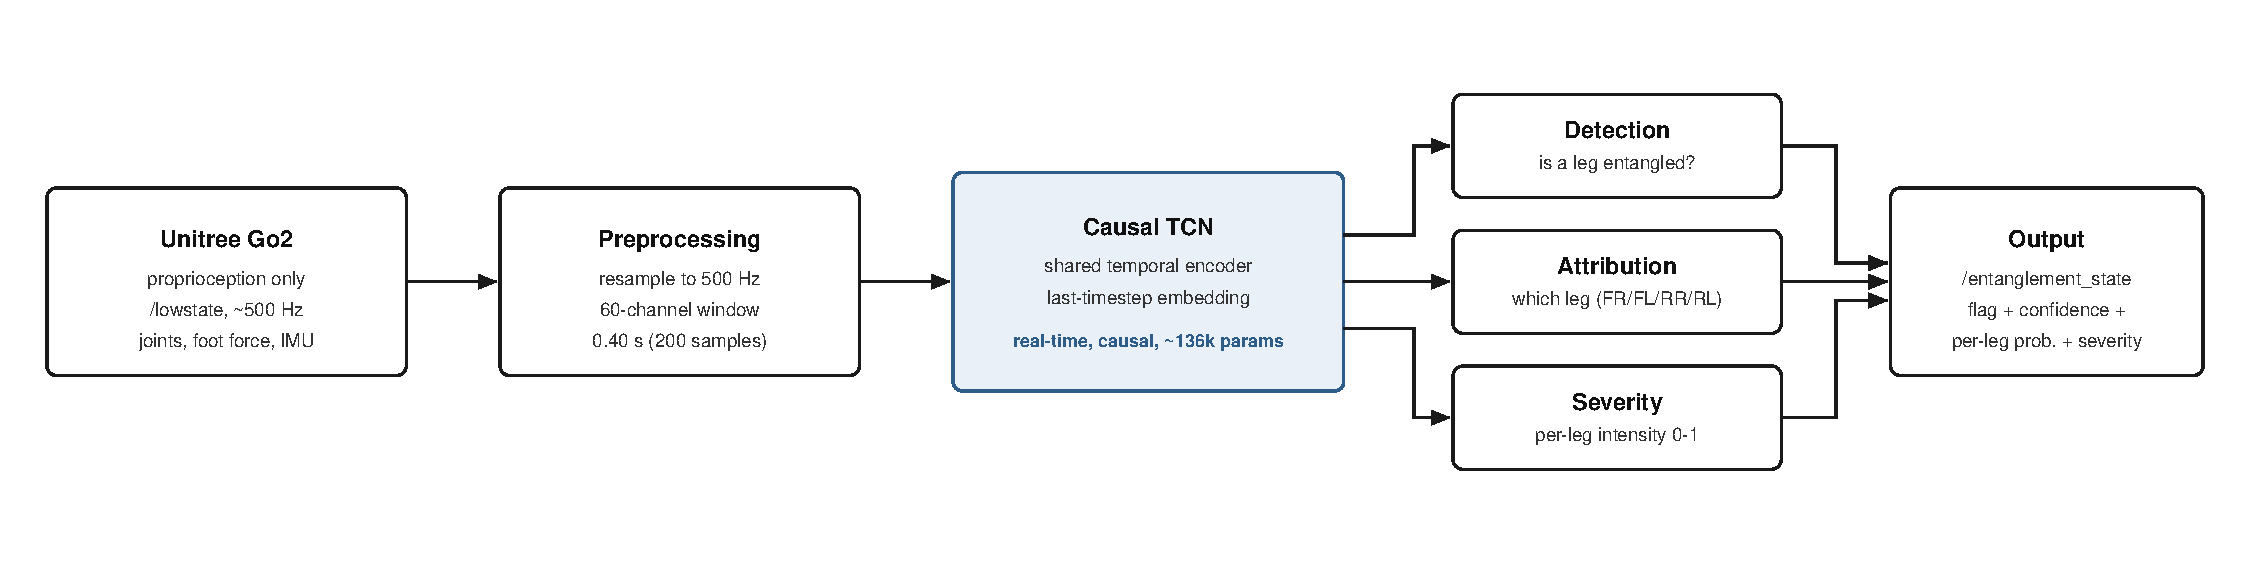
\includegraphics[width=\textwidth]{figures/fig1_system.pdf}
\caption{Overall system architecture. Proprioception from the Go2 is windowed and passed through a
shared causal TCN encoder whose three heads answer whether a leg is entangled, which leg, and how
severely; the result is published as a single state estimate.}
\label{fig:system}
\end{figure*}

\section{Related Work}

The closest prior work is Yim et al.~\cite{yim2023entanglement}, which detects leg entanglement from proprioception and, when a leg snags, executes a disentanglement maneuver as that leg advances through its swing phase, succeeding in 14 of 16 laboratory trials and in outdoor tests. It establishes entanglement as a real and tractable failure mode, but it also leaves clear gaps. Detection is largely rule-based and reactive, tied to gait-phase timing rather than to a learned temporal model; the output is effectively a binary trigger, with no attribution of which leg is caught and no measure of how strongly it is held; and sensing is fused with the reactive control loop rather than exposed as a reusable estimate. We keep the proprioceptive premise but address these gaps: we integrate evidence over a fixed $0.40$~s window with a learned causal model instead of an instantaneous rule, we emit structured outputs (which leg, and a calibrated per-leg severity in $[0,1]$), and we treat detection as a self-contained perception problem that publishes a state estimate, decoupled from any actuation policy. The contrast is in what is inferred and how it is reported, not in closing a control loop.

Proprioceptive learning is otherwise well established for legged systems, from locomotion policies that transfer to hardware~\cite{hwangbo2019learning,lee2020learning} to probabilistic contact and event estimation~\cite{camurri2017contact,bledt2018contact}. Entanglement differs in kind: it is an externally imposed kinematic constraint, applied at an unpredictable time and place, that must be localized to a leg and graded by how strongly it resists, rather than classified as contact versus no contact. For the model we build on temporal convolutional networks~\cite{bai2018tcn} and the dilated causal convolutions of WaveNet~\cite{oord2016wavenet}, whose causality and stride-spanning receptive field suit an at-every-timestep detector that must run online. Finally, because a detector is only usable if its confidence maps to a trustworthy threshold, we apply temperature scaling~\cite{guo2017calibration,niculescu2005predicting}, mainly to de-saturate probabilities that would otherwise pin near $1.0$.

\section{Methodology}
\label{sec:method}
\subsection{Data Collection}

Our data come from a single Unitree Go2, whose onboard proprioception is published on the ROS~2 topic \texttt{/lowstate}~\cite{macenski2022ros2,unitree_go2}. We recorded this stream while running scripted locomotion scenarios and stored each as a comma-separated-value (CSV) log. Positive scenarios walk the robot and then drive one leg into a physical entanglement (a wire or a hand) before releasing it; negative scenarios contain no entanglement. We also scripted a \texttt{Lock} condition, the rigid stance the robot holds right after standing up, because it produces large, sustained joint torques with almost no motion and thus superficially resembles a snag; including it as a labeled negative teaches the model to tell a held stance from a genuine entanglement.

Logging is event-driven, so the effective rate is non-uniform, ranging from roughly $410$ to $500$~Hz (median near $483$~Hz); we keep this raw timing and defer resampling to the feature stage. The corpus is $25$ recordings totaling $159{,}001$ labeled rows, each with $51$ columns in three sensor groups plus a label. The motor group holds $36$ values: four legs, each with hip, thigh, and calf joints reporting position $q$, velocity $dq$, and torque $\tau$. The next group is the four foot-contact forces, and the last is the inertial measurement unit (roll, pitch, yaw, three gyroscope and three accelerometer axes). A final \texttt{Status} column carries the phase label. Table~\ref{tab:dataset} summarizes these groups.

We labeled the recordings by hand. Because each scenario was scripted, we knew when an entanglement began and ended, and we combined those timestamps with per-joint torque plots (the more reliable cue, since a snag shows a distinctive sustained resistive torque) to mark the exact rows of each event. Each row receives one of the phase labels \texttt{Walking}, \texttt{Entangled}, \texttt{Stop}, \texttt{Lock}, or blank, and the affected leg of a positive recording is encoded in its filename.

Of the $25$ recordings, $15$ are positive (one contiguous entangled event each) and $10$ are negative. The positive events are unevenly distributed across legs: grouping by affected leg gives seven recordings for the rear-right, five for the rear-left, four for the front-left, and only three for the front-right. The front-right leg is therefore under-represented, which constrains how confidently its per-leg behavior can be estimated and resurfaces in the per-leg results (Table~\ref{tab:perleg}). Splits are formed at the level of whole recordings (Sec.~\ref{sec:method} explains why), assigning $16$ recordings to training, $4$ to validation, and $5$ to test; the held-out test set is \texttt{back\_left\_hand2}, \texttt{back\_right\_wire1}, \texttt{front\_left\_hand2}, and \texttt{front\_both\_wire2}, with \texttt{go2\_lowstate\_lock\_stop} as the negative.
\begin{table}[t]
\centering
\caption{Dataset composition. 25 recordings, 159{,}001 labeled rows, logged non-uniformly
($\approx$410--500\,Hz, median $\approx$483\,Hz) and resampled to 500\,Hz at the feature stage. The
affected leg is encoded in the file name.}
\label{tab:dataset}
\footnotesize
\begin{tabular}{@{}lccl@{}}
\toprule
Scenario & \#Rec. & Affected & Interaction \\
\midrule
\texttt{back\_both}  & 2 & RR, RL & wire \\
\texttt{back\_left}  & 3 & RL     & hand / wire \\
\texttt{back\_right} & 3 & RR     & hand / wire \\
\texttt{front\_both} & 2 & FR, FL & wire \\
\texttt{front\_left} & 2 & FL     & hand \\
\texttt{front\_right}& 1 & FR     & wire \\
\texttt{back\_right} (at rest) & 2 & RR & wire \\
\midrule
\texttt{walking} & 5 & --- & normal gait \\
\texttt{stop}    & 3 & --- & standing \\
\texttt{lock\_stop}, \texttt{walk\_stop\_back} & 2 & --- & Lock / backward \\
\midrule
\textbf{Total} & \textbf{25} & \multicolumn{2}{l}{\textbf{15 positive / 10 negative}} \\
\bottomrule
\end{tabular}
\end{table}

\subsection{Feature Engineering}
\label{sec:feat}

A temporal convolution assumes a fixed sampling interval: a filter of a given length always spans the same number of milliseconds, and dilations correspond to fixed time offsets. Fed the non-uniform raw logs, a 200-sample window would cover a different physical duration in each recording and the learned filters would mean different things across files. We therefore resample every recording onto a common 500~Hz grid (a 2~ms step): continuous signals by linear interpolation, and the categorical \texttt{Status} label by nearest-neighbor, which preserves each row's discrete phase rather than blending two labels.

The result is a 60-channel per-timestep representation (Table~\ref{tab:features}). Forty-eight are raw: the 36 motor channels (four legs $\times$ \{hip, thigh, calf\} $\times$ \{$q,dq,\tau$\}), the 4 foot-contact forces, and 8 IMU channels. We keep roll, pitch, and the gyroscope and accelerometer axes but drop yaw, which integrates the yaw rate with no fixed reference on level ground and would tie the features to an arbitrary heading.

The remaining 12 channels are engineered, three per leg, to encode the mechanical signature of a snag. When a leg catches, the motor keeps commanding motion but the limb cannot move, so the joint develops a large torque while its velocity stays near zero; a raw torque channel alone misses this, because normal fast strides also produce large torques. The first feature isolates the resistive (downward) part of the thigh torque:
\begin{equation}
\texttt{thigh\_tau\_down} = \max(0,\, -\tau_{\text{thigh}}).
\end{equation}
The second expresses the ``high torque, little motion'' signature directly, with $\varepsilon = 0.05$ keeping the ratio finite when the leg is nearly still:
\begin{equation}
\texttt{thigh\_down\_effort} = \frac{\texttt{thigh\_tau\_down}}{|dq_{\text{thigh}}| + \varepsilon}.
\end{equation}
It is large when the thigh pushes hard while barely moving and small during ordinary swinging. The third sums the absolute torque across the leg's joints,
\begin{equation}
\texttt{tau\_sum} = \sum_{j \in \{\text{hip},\,\text{thigh},\,\text{calf}\}} |\tau_j|,
\end{equation}
a per-leg effort measure that helps attribute an event to the correct limb. All 60 channels are then z-score standardized using statistics estimated on training rows only, so nothing about the held-out recordings leaks into the normalization.

Finally, the network reads a sliding window of 200 samples, which at 500~Hz is 0.40~s, about one trot stride: shorter than a stride it could mistake a step's normal high-torque phase for a snag, whereas a full stride separates a passing spike from a sustained resistance. Training advances the window by a hop of 25 samples for many decorrelated examples; evaluation uses a dense hop of 1 so every timestep yields a prediction, matching the online detector. A window is labeled positive when at least $50\%$ of its rows are \texttt{Entangled}; windows in the ambiguous band ($0.2$--$0.5$) are excluded from training but kept for evaluation, and \texttt{Stop}/\texttt{Lock}-dominated windows are negatives.
\begin{table}[t]
\centering
\caption{The 60-channel input representation. Motor torque is the estimated joint torque $\tau$.}
\label{tab:features}
\footnotesize
\begin{tabular}{@{}llc@{}}
\toprule
Group & Channels & Count \\
\midrule
Motor & 4 legs $\times$ \{hip, thigh, calf\} $\times$ \{$q,\dot q,\tau$\} & 36 \\
Foot force & one per leg & 4 \\
IMU & roll, pitch, gyro$_{xyz}$, acc$_{xyz}$ (yaw dropped) & 8 \\
Engineered & per leg: 3 physics features (Sec.~\ref{sec:feat}) & 12 \\
\midrule
\textbf{Total} & & \textbf{60} \\
\bottomrule
\end{tabular}
\end{table}

\subsection{Machine Learning Pipeline}

Every 0.40\,s window (200 samples at 500\,Hz, 60 channels) must yield three answers at once: whether any leg is entangled, which leg, and how severe. The detector also faces a hard operational constraint: at time $t$ it sees a stream ending at the current instant and can never look ahead. We use a temporal convolutional network (TCN) \cite{bai2018tcn} because it meets this constraint by construction, processes a whole window in parallel rather than step by step, and extends its temporal reach cheaply through dilation. Figure~\ref{fig:tcn} shows the architecture; Table~\ref{tab:hparams} lists the hyperparameters.

Causality is enforced by left-padding: each convolution is padded only on the past side, so the output at $t$ depends on $\{x_{t-k},\dots,x_t\}$ and nothing later, following the causal-convolution idea of WaveNet \cite{oord2016wavenet}. The payoff is that the model trained offline on complete windows is numerically the same function that runs online on a growing buffer, with no train--test discrepancy from look-ahead (verified empirically below).

A causal convolutional stem lifts the 60 input channels to 64, and five residual blocks follow with dilation factors $1,2,4,8,16$. Dilation inserts gaps between kernel taps, so a fixed kernel size covers an exponentially longer span as blocks stack, reaching far back in time without a matching growth in parameters. With kernel size 3 the receptive field is 127 samples (254\,ms), inside the 0.40\,s window, so the last position has seen most of a trot stride before deciding. Each block applies a causal convolution, a GELU \cite{hendrycks2016gelu}, a second causal convolution, another GELU, dropout 0.1, and an identity skip connection; both convolutions use weight normalization \cite{salimans2016weightnorm}. The skip lets each block learn a refinement of its input, which stabilises training of the stack.

We read out only the last-timestep embedding, a single 64-D vector: at deployment the decision of interest is the one \emph{now}, and the last position is exactly the one whose receptive field ends at the present sample. Three linear heads follow: detection (one logit), leg attribution (four independent logits, since multiple legs may be affected), and intensity (four values). The network has 136{,}393 parameters, small enough to ship as a half-megabyte model.

The tasks share one weighted objective. Detection and leg attribution use binary cross-entropy; intensity uses a Huber loss, which is robust to outliers. Detection and leg are weighted equally, and intensity is down-weighted as an auxiliary term:
\begin{equation}
\mathcal{L} = 1.0\,\mathrm{BCE}_{\text{det}} + 1.0\,\mathrm{BCE}_{\text{leg}} + 0.3\,\mathrm{Huber}_{\text{int}} .
\end{equation}
The intensity Huber ($\delta=0.1$) is computed against a physics pseudo-target, not a human label, and affected-leg elements are up-weighted $3{:}1$. This is an up-weight, not a hard mask: since most legs carry a target of zero, flat weighting would let ``predict zero everywhere'' dominate. The head therefore weakly tracks the physics target, which remains authoritative at inference. Class imbalance is handled by a class-balanced sampler plus a capped positive-class weight in each cross-entropy. Optimization uses AdamW \cite{loshchilov2019adamw} with a cosine schedule over 30 epochs (Table~\ref{tab:hparams}).

Severity is reported through a physics-grounded index, because no ground-truth severity labels exist. Per leg it combines a confidence gate $g$ (the per-leg entanglement probability, so the index is near zero when the leg is not flagged), a deviation term $d$ (the Mahalanobis distance of the window's per-leg features from the walking distribution, fit on training walking data only), and a resistive-effort term $r$ (mean downward thigh torque divided by thigh speed, high when a leg pushes hard yet barely moves):
\begin{equation}
I_{\text{leg}} = g\,\sqrt{d\,r},
\end{equation}
calibrated to $[0,1]$ and reported as an index, not a measured force. The deployed value blends the network head and this physics index in equal parts.

A TCN suits these requirements better than the alternatives. A recurrent network is sequential, trains one step at a time, and is awkward to keep strictly causal-equivalent between offline and online use; a gradient-boosted ensemble has no native notion of time and would need hand-built window summaries, discarding the temporal structure that separates a transient snag from a steady stance.
\begin{figure*}[t]
\centering
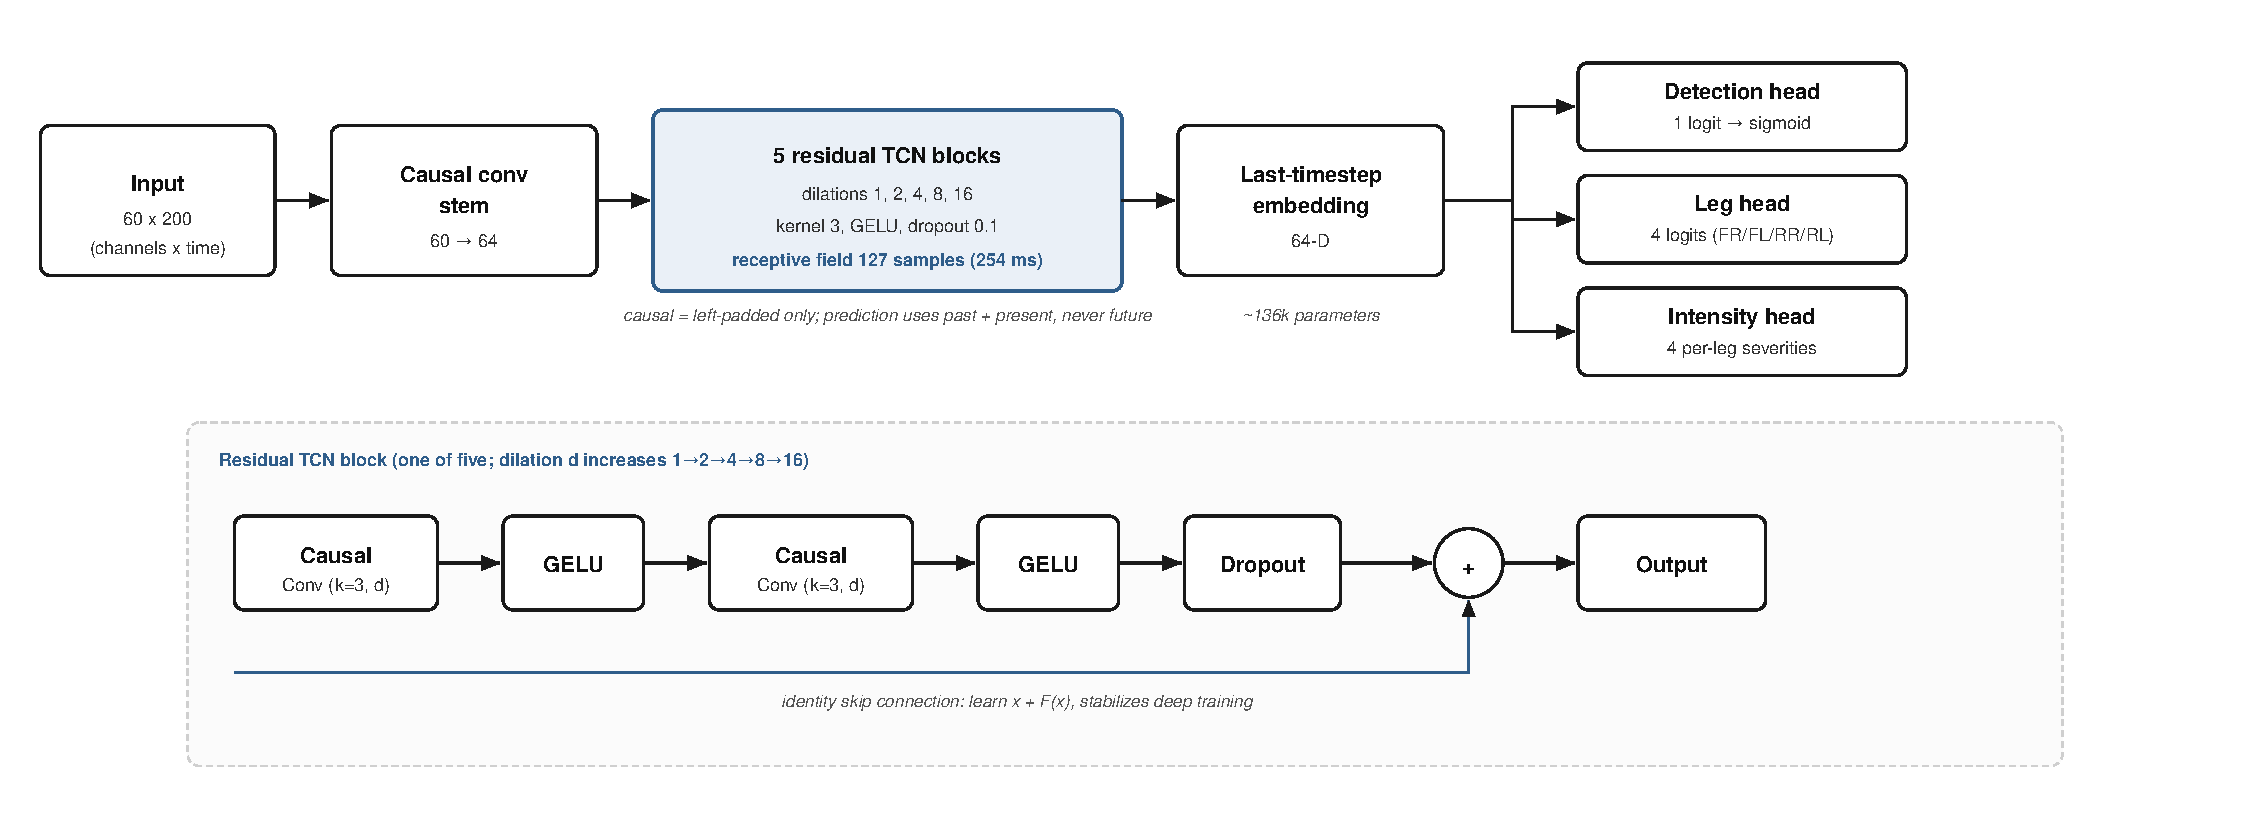
\includegraphics[width=\textwidth]{figures/fig4_tcn.pdf}
\caption{Multi-task causal TCN. A causal convolutional stem feeds five dilated residual blocks; the
last-timestep 64-D embedding drives the detection, leg-attribution, and intensity heads. The inset
shows one residual block.}
\label{fig:tcn}
\end{figure*}
\begin{table}[t]
\centering
\caption{Model and training configuration.}
\label{tab:hparams}
\footnotesize
\begin{tabular}{@{}ll@{}}
\toprule
Item & Value \\
\midrule
Window / hop (train, eval) & 200 (0.40\,s) / 25, 1 \\
Resample rate & 500\,Hz \\
Encoder width / blocks & 64 / 5 \\
Dilations; kernel; dropout & 1,2,4,8,16; 3; 0.1 \\
Receptive field & 127 samples (254\,ms) \\
Parameters & 136{,}393 \\
Loss weights (det / leg / int.) & 1.0 / 1.0 / 0.3 \\
Intensity Huber & $\delta{=}0.1$, affected-leg $3{:}1$ up-weight \\
Optimizer & AdamW, lr $10^{-3}$, wd $10^{-4}$ \\
Schedule; batch; epochs; seed & cosine; 256; 30; 1234 \\
Sampler & class-balanced, rare-leg up-weighted \\
\bottomrule
\end{tabular}
\end{table}

\subsection{Runtime Architecture}
\label{sec:runtime}

On the robot the detector is a ROS~2 node that turns the raw telemetry stream into a published
state estimate. The same preprocessing and model serve offline training and online inference, and only the exported ONNX model together with the saved normalization and calibration statistics cross the deploy boundary.

The node subscribes to \texttt{/lowstate} with \texttt{BEST\_EFFORT} quality of service. Reliable
delivery would add retransmission latency to a stream that arrives hundreds of times per second, and
a dropped proprioceptive sample matters far less than a late one, so trading guaranteed delivery for
low latency is the right call. Each message is adapted into the 48 raw signals the model expects and
pushed into a 200-sample circular ring buffer; the buffer holds memory and per-sample cost constant,
since the oldest sample is overwritten as each new one arrives rather than reallocating a growing
window. Once the buffer is full it is expanded to the 60-channel representation and normalized with
the statistics saved at training time.

Inference runs through ONNX Runtime rather than PyTorch. The exported graph loads faster, uses less
memory, and removes the training-framework dependency from the robot, which matters on a constrained
onboard target~\cite{onnxruntime,macenski2022ros2}. The detection logit is passed through a sigmoid
and, separately, through a temperature-scaled sigmoid ($T=5.918$) to produce the reported confidence;
the per-leg severity is the equal-weight blend of the network head and the physics index. Raw network
predictions flicker from sample to sample, so a detection is latched only after the raw probability
stays above threshold for 75~ms. That short temporal debounce suppresses isolated spikes without
noticeably delaying a genuine alarm. Per-leg thresholds then name the affected leg, with the
rear-right threshold raised to 0.9 because that leg was the most prone to false positives; the others
use 0.5. The node publishes
\texttt{/entanglement\_state}, carrying the debounced flag, the calibrated confidence, four per-leg
probabilities, four per-leg severities, and the name of the alarm leg.

\subsubsection{Stationarity gate}
One failure mode surfaced only in testing. When the robot walks, stops, and then stiffens into the
rigid Lock stance it holds after standing up, the ring buffer still contains the tail of the walking
motion, and the detector can briefly report entanglement for a robot that is simply standing still.
The gate that fixes this watches the mean absolute joint velocity: when it falls below 0.30~rad/s for
100~ms the robot is treated as stationary, and the node clears the ring buffer, resets the debounce
counter, and arms a 300~ms suppression window that ignores the transient while gait is re-acquired.
The gate is edge-triggered, so it acts once on the transition rather than continuously. It is disabled
in the research configuration so that the evaluation pipeline is byte-identical to the deployed one,
and enabled only on the robot.

\section{Experimental Setup}

Evaluation is dominated by one fact: entanglements are rare, contiguous events, and the 25 recordings differ in gait and affected leg. A window-level random split would put near-identical neighbouring windows from one recording on both sides of the partition, leaking information and inflating every score, so all protocols group by whole recording. We report two. The first is a fixed leakage-safe split of 16 training / 4 validation / 5 test recordings (the five test recordings are four positive and one negative); normalization statistics and the walking reference distribution for the severity index are fit on training rows only. The second, our headline generalization protocol, is leave-one-recording-out (LORO) cross-validation over the 15 positive recordings: each fold holds out one positive recording, trains on the rest, and we report the mean and standard deviation of the per-fold $F_1$. Its variance across folds is itself informative. Both use dense evaluation, sliding the 200-sample window with hop 1 so a decision is produced at every timestep, matching how the runtime consumes \texttt{/lowstate}; this also scores the hard event boundaries.

Metrics are standard, computed on the dense windows. Precision, recall, and their harmonic mean $F_1$ summarize the detection head; PR-AUC and ROC-AUC are threshold-free, with PR-AUC the more meaningful here because positives are rare. For attribution we use multi-label exact-match, which counts a window correct only when the predicted set of entangled legs equals the true set exactly. As a non-learned reference, a thigh-torque heuristic fires when a leg's resistive torque is high; we evaluate it under the identical dense, grouped protocol on the same windows, so the comparison in Table~\ref{tab:detection} isolates the value of the learned model.

Two further analyses use the same protocol. For the feature ablation we retrain from scratch on channel subsets (engineered only, raw only, raw+engineered without foot contacts, without the IMU, and the full set) and re-run LORO, so the resulting change in $F_1$ reflects each group's marginal contribution rather than a post-hoc importance estimate. For calibration we report the Brier score, the expected calibration error (ECE), and saturation (the fraction of raw probabilities pinned near $1.0$); temperature scaling \cite{guo2017calibration,niculescu2005predicting} is applied to de-saturate the output so a usable operating threshold exists, and we report the effect without assuming de-saturation implies better reliability. Latency is measured on the deployment ONNX runtime \cite{onnxruntime}, pinned to a single CPU thread, timing the per-window forward pass plus post-processing; this is a development-machine benchmark, not a measurement on the Go2's onboard computer.

\section{Results}

Every number below comes from offline replay of recorded logs; we make no claim about live on-robot detection performance.

\subsection{Detection on the held-out test split}
Table~\ref{tab:detection} compares the TCN against a rule-based baseline that thresholds thigh torque, under an identical protocol on the same five test recordings. The TCN reaches precision $0.799$, recall $0.818$, and $F1 = 0.809$, with $\text{PR-AUC} = 0.808$ and $\text{ROC-AUC} = 0.956$. The baseline attains comparable precision ($0.735$) but collapses on recall ($0.131$), for $F1 = 0.222$: a fixed threshold catches only the most violent snags and misses the many entanglements that manifest as sustained resistive effort rather than a single spike. The gap in $F1$ ($0.809$ vs.\ $0.222$) and in multi-label exact-match ($0.908$ vs.\ $0.106$) is the central detection result. At the operating point (raw threshold $0.9999$) the errors are TP $2833$, FP $712$, FN $630$, TN $9126$, roughly balanced between false alarms and misses; the ROC-AUC of $0.956$ confirms strong ranking, while the lower PR-AUC of $0.808$ is expected under the heavy class imbalance.

\subsection{Generalization across recordings (LORO)}
Because a single split samples only a handful of events, we also run leave-one-recording-out (LORO) cross-validation, retraining with each positive recording held out in turn. Across the 15 folds in Fig.~\ref{fig:loro}, $F1 = 0.807 \pm 0.142$, closely tracking the test-split value and indicating the split is representative rather than lucky. The spread is uneven: the weakest folds are the front-right recording (the least represented leg) and the deployment recordings that capture entanglement while the robot stands at rest, a regime that differs most from the walking-dominated remainder.

\subsection{Per-leg attribution}
Naming the affected leg is the other half of the task. Table~\ref{tab:perleg} gives per-leg detection on the test split. Recall is high across all four legs (FR/FL $1.000$, RR $0.959$, RL $0.916$), so genuine events are rarely missed; the differences are in precision. Front-right shows a clear trade-off, recovering every event (recall $1.000$) at precision $0.467$ for $F1 = 0.636$, the lowest of the four. This matches the LORO finding: FR has the fewest positive appearances, so the model fires readily on it. The other legs are stronger (FL $0.845$, RL $0.823$, RR $0.700$).

\subsection{Calibration}
A detector's probabilities are only useful if a threshold can be set from them. The raw network is over-confident: about $27\%$ of window probabilities pin near $1.0$, which forces the false-alarm-controlled threshold to clamp at $0.9999$. Temperature scaling with $T = 5.918$ de-saturates the output and lets the operating threshold move to a usable $0.963$. The effect on scoring is mixed: the Brier score improves slightly ($0.128 \to 0.118$), but the expected calibration error does \emph{not} ($0.134 \to 0.156$). Scaling therefore buys a de-clamped, interpretable threshold, not better calibration in the ECE sense.

\subsection{Feature ablation}
Retraining with feature groups removed and re-running LORO gives the change in $F1$ relative to the full 60-channel set. Raw kinematics are essential: the engineered channels alone drop $F1$ by $0.13$. The engineered channels still earn their place (raw-only sits $0.03$ below the full set), foot contacts matter little ($-0.01$), and the IMU is effectively redundant (dropping it leaves $F1$ unchanged to two decimals). Joint position, velocity, and torque do the work; the snag-signature channels add a small margin.

\subsection{Deployment robustness}
Offline test metrics miss failure modes that appear on specific field recordings, so we retrained with targeted data augmentation and measured per-phase firing rates before (v1) and after (v2); Fig.~\ref{fig:field} summarizes them. Four false-fire modes fell to essentially zero: Lock firing on \texttt{lock\_stop} ($0.8 \to 0.0$) and \texttt{walk\_stop\_back}-Lock ($4.7 \to 0.0$), rear-right firing while stopped ($100 \to 0$), and backward-walking firing ($9.7 \to 0$). On the dedicated front-right event, binary firing rose from $30.7\%$ to $78.5\%$ and correct-leg firing from $4\%$ to $100\%$. This was not free: the hard-negative recordings cost a little accuracy on the original, easier protocol in exchange for removing the field false-fire modes.

\subsection{Runtime}
On the deployment ONNX runtime on a single CPU thread (a development-machine benchmark, not the Go2's onboard computer), mean and median latency are about $1.0$~ms/window with a p95 near $1.3$~ms, under the $2.0$~ms budget at $500$~Hz; the model is about $0.5$~MB. The runtime reproduces the research pipeline to within $\leq 3.8\times10^{-7}$ (detection), $6.3\times10^{-7}$ (per-leg), and $2.1\times10^{-7}$ (intensity), so the offline metrics transfer to the deployed node to roughly $10^{-6}$.
\begin{table}[t]
\centering
\caption{Detection on the held-out test split (raw threshold 0.9999). Both detectors are scored
under the identical protocol.}
\label{tab:detection}
\footnotesize
\begin{tabular}{@{}lcc@{}}
\toprule
Metric & Causal TCN & Rule-based (thigh torque) \\
\midrule
Precision       & \textbf{0.799} & 0.735 \\
Recall          & \textbf{0.818} & 0.131 \\
F1              & \textbf{0.809} & 0.222 \\
PR-AUC          & \textbf{0.808} & 0.639 \\
ROC-AUC         & \textbf{0.956} & 0.830 \\
Leg exact-match & \textbf{0.908} & 0.106 \\
\bottomrule
\end{tabular}
\end{table}
\begin{figure*}[t]
\centering

\includegraphics[width=\textwidth]{figures/loro_folds.pdf}
\caption{Leave-one-recording-out cross-validation (15 folds). Bars are per-fold detection F1; the
line and band are the mean and $\pm$one standard deviation. The weakest folds are the
under-represented front-right and rear-right stop/intensity recordings.}
\label{fig:loro}
\end{figure*}
\begin{table}[t]
\centering
\caption{Per-leg attribution on the test split.}
\label{tab:perleg}
\footnotesize
\begin{tabular}{@{}lccc@{}}
\toprule
Leg & Precision & Recall & F1 \\
\midrule
FR & 0.467 & 1.000 & 0.636 \\
FL & 0.731 & 1.000 & 0.845 \\
RR & 0.551 & 0.959 & 0.700 \\
RL & 0.748 & 0.916 & 0.823 \\
\bottomrule
\end{tabular}
\end{table}
\begin{figure*}[t]
\centering

\includegraphics[width=\textwidth]{figures/field_issues.pdf}
\caption{Deployment robustness from targeted data augmentation. (a) Three false-firing modes fall to
zero. (b) Front-right detection rises from near zero to full. Values are per-phase firing percentages
on the named recordings.}
\label{fig:field}
\end{figure*}

\section{Conclusion}
We presented a compact causal temporal convolutional network that reads only proprioception from a Unitree Go2 and answers three questions at once: whether a leg is entangled, which of the four legs (FR/FL/RR/RL) is affected, and how severe the entanglement is on a $[0,1]$ scale. The model is small (roughly $136$k parameters, about $0.5$~MB) and its strictly left-padded convolutions use only past and present samples, so a single forward pass runs in about $1$~ms per window on a single CPU thread, under the $2$~ms budget at $500$~Hz. Evaluation was leakage-safe by grouping whole recordings across the train/validation/test split, and leave-one-recording-out cross-validation over $15$ folds gave $\mathrm{F1}=0.807\pm0.142$ (Figure~\ref{fig:loro}); on the held-out test split the detector reached $\mathrm{F1}=0.809$ and $\mathrm{ROC\text{-}AUC}=0.956$, far ahead of the thigh-torque rule-based baseline at $\mathrm{F1}=0.222$ under an identical protocol (Table~\ref{tab:detection}). A targeted, data-centric augmentation step suppressed the field false alarms we observed on stationary and backward-walking segments while recovering the under-represented front-right event (Figure~\ref{fig:field}). Two limitations bound these claims: every detection metric is offline, computed on recorded-CSV replay rather than live on-robot operation, and the reported severity is a physics-grounded, calibrated index rather than a measured contact force, since no ground-truth severity labels exist.

\clearpage
\bibliographystyle{IEEEtran}
\bibliography{references}

\end{document}
